% https://www.overleaf.com/project/5ecb71b63aa15c0001db6036

\documentclass[a4paper,12pt]{article}
% make four margins to be 1 inch
\usepackage{fullpage}
% use UTF8 encoding
\usepackage[utf8]{inputenc}
% use KoTeX package for Korean 
\usepackage{kotex}
% for the fancy \koTeX logo
\usepackage{kotex-logo}
\usepackage[onehalfspacing]{setspace}

% for multiple columns
\usepackage{multicol}

\usepackage{graphicx}
\graphicspath{ {./image/} }

% add an information about the author of a poem
\newcommand{\attrib}[1]{%
  \nopagebreak{\raggedleft\footnotesize #1\par}}


\begin{document}

\title{}
\author{}
\date{}
\setstretch{1.4}
\maketitle
\newpage
\tableofcontents
\newpage

% 11111111111111111
\section{구조적 개발방법론}

\subsection{개요}
\subsubsection{등장 배경}
- 소프트웨어 개발의 증가로 \textbf{소프트웨어 위기(Software Crisis)}\footnote{소프트웨어 위기: SW의 기능을 변경하거나, 하나의 SW를 다른 SW와 연계하는 비용이 급증하는 현상}의 발생.
\newline
- \textbf{'GOTO 논쟁'}: 프로그램을 짜는 것에 있어서 GOTO문은 판독성을 해치고 복잡한 구조를 만드므로 사용하지 말아야 한다는 주장이 제기됨.
\newline
- SW를 체계적으로 개발하고 유지 보수하는 \textbf{소프트웨어 공학(Software Engineering)}의 개념이 도입됨.

\subsubsection{원리}
- GOTO문 대신에 \underline{'순차(Sequencing) → 선택(Selection) → 반복(Iteration)'}을 활용해 모든 Logic을 해결함.
\newline
- Top-Down 형태의 하향화 구조로 진행됨.
\newline

\subsection{사용 개념}
- \textbf{추상화(Abstraction)}: 세부사항을 모두 쓰지 않고, 단순하게 개념화시켜 표현하는 것.
\newline
- \textbf{정보 은닉(Information Hiding)}: 캡슐화시켜 다른 모듈의 세부 내용에 영향을 끼치지 않게 Data \& Method를 숨기는 것.
\newline
- \textbf{구조화(Structure)}: 계층적인 구조를 부여하고, 상위 Module이 하위 Module을 활용하게 하는 것.
\newline
- \textbf{단계적 상세화(Stepwise Refinement)}: 하향식으로 진행하면서 점차 내용을 구체화시키는 것.
\newline
- \textbf{모듈화(Modulization)}: 하나의 System을 Sub-System, Program, Module 등으로 구분하여 정의하고 개별적으로 설계하는 것.
\newline

\subsection{특징}
- 구조중심으로 분석하고, 분석 절차가 정형화되어있음.
\newline
- 설계 문서화, 모듈화를 위해 하향식 분할\footnote{ex) 폭포수 모델} → 자료흐름을 지향하는 기법을 사용함.
\newline
- 사용자의 요구사항, 문서화 등을 기반으로 개발함.
\newline
- 도형 중심의 분석 도구를 사용 → 한 눈에 파악하기에 용이함.
\newline
- \underline{분할과 정복, 추상화의 원칙}에 기반함.
\newline

\subsection{분석과 프로세스 기법}
\subsubsection{요구사항 분석}
- 사용자의 요구를 파악하고, 요구사항을 명세화시킴.
\newline
- 데이터, 환경, 기능 등을 종합적으로 분석함.

\subsubsection{구조적 분석}
- 종합적으로 분석한 내용을 토대로 \textbf{자료 흐름도(DFD, Data Flow Diagram)} 작성.

- DFD: 자료가 프로세스를 따라 \underline{흐르며 변환되는 과정을 표시}한다.

- 추상화로 주요 내용을 명시하고, 하향식 분할 정복으로 기능을 분해한다.

- 최하위 단계의 Logic을 사용하는 소단위 명세서를 작성한다.
\newline
- DFD에서 명시하는 데이터 상세 내용은 \textbf{자료 사전(DD, Data Dictionary)}에서 표시됨.

- DD: \underline{자료의 의미, 단위, 값, 정의 등}을 포함한다.

- DFD의 자료 저장소를 구체적으로 명시하며 서로 상호 보완적인 분석 도구이다.
\newline
- 구조적 언어, 의사 결정도, 의사 결정표, N-S 도표 등 사용.

\subsubsection{구조적 설계}
- SW Module 중심으로 설계함.
\newline
- DFD 중심, 독립성과 결합성 고려, 재활용성 좋은 모델의 설계.

\subsubsection{구조적 프로그래밍}
- \textbf{'순차(Sequencing) → 선택(Selection) → 반복(Iteration)'}의 논리 구조로 구성된다.

\newpage
% 222222222222222
\section{정보공학 개발방법론}

\subsection{개요}
\subsubsection{등장 배경}
- \underline{Relational DataBase (RDB)} 출현 → 단위업무에서 전사적 규모의 \underline{'통합 시스템'}으로의 변화가 요구됨.
\newline
- 기업 전체 조망과 데이터 통합에 어려움이 발생함 → 기업적인 새로운 정보 시스템의 개발이 필요함.
\newline
- 컴퓨터 업무 활성화, 업무 기능, 정보 기술 발달 등에 따른 구조적 개발방법론의 한계가 드러남.

\subsubsection{정의}
- 계획/분석/설계의 전 과정을 정형화시킨 절차 및 방법론임.
\newline
- \textbf{Architecture Definition}을 통해 업무에서 정보의 효율적인 사용이 가능함.
\newline
- 기업에 필요한 정보/업무를 분석/설계하는 공학적 기법을 사용했고, 작업절차 체계화시킴.
\newline
- 대표적으로 \textbf{'프로토타입 모델링(Prototype Modeling)'}이 이에 해당함.
\newline

\subsection{특징}
\subsubsection{기업중심}
- 적용 대상이 기업의 비즈니스 시스템임.
\newline
- \textbf{SIS(Strategic Information System, 전략정보시스템)}에 초점을 둠.

- SIS: \underline{컴퓨터망, DB 중심, 최근에는 가치 창조에 초점}을 두는 전략임.\footnote{실례로는 금융 기관 온라인 시스템, 항공 회사 좌석 예약, 슈퍼마켓 등에서의 판매 시점 관리 등이 있다.}

- 기업의 전략을 실현해 경쟁 우위를 확보하자는 목적으로 활용, 이익에 직접 영향을 줄 수 있는 전략계획(시장점유율 향상, 매출신장, 경영전략 등)에 도움을 주는 정보 시스템

- 정보 시스템이 활용되는 방안: 제품/서비스 내용 변경, 고객과의 관계 확고화, 공급업자와의 전략적 우위 확보, 효율적인 내부 관리 및 통제

\subsubsection{정보전략계획(ISP) 중심}
- 정보공학 4단계 중 \underline{가장 처음으로}, 경영층의 요구와 견해를 시스템에 반영함.
\newline
- 전사적 관점에서 정보시스템, 정보관리 체계 및 전략계획을 수립함.
\newline
\newline
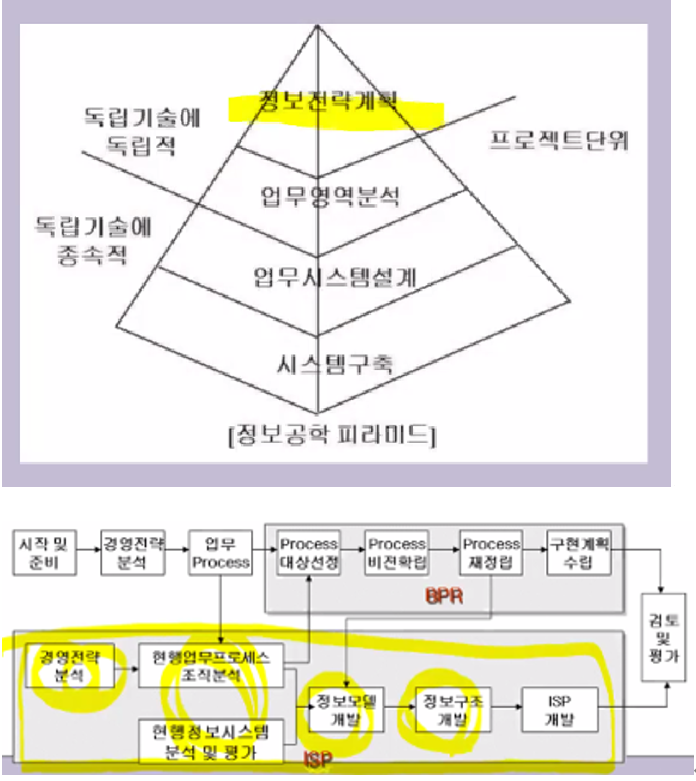
\includegraphics[scale=0.8]{21}
\newline
\newline
- 경영전략분석 → 현행 업무 프로세스 및 조직의 분석 → 현행 정보시스템 분석 및 평가 → 정모 모델 및 Architecture 개발 → SIS 수립 의 단계를 거침.

\subsubsection{데이터 중심}
- 데이터는 잘 변하지 않으므로, 유지보수를 줄이고 잦은 변화에 적극적으로 대응함.

\subsubsection{분할과 정복}
- 문제의 영역을 세분화하면서 Top-Down 방식으로 완성함.

\subsubsection{공학적 접근}
- Case Tool, Modulization, Diagram ...

\subsubsection{사용자 참여}
- 초기 단계부터 사용자의 적극적인 참여와 피드백을 반영함.
\newline

\subsection{프로세스}

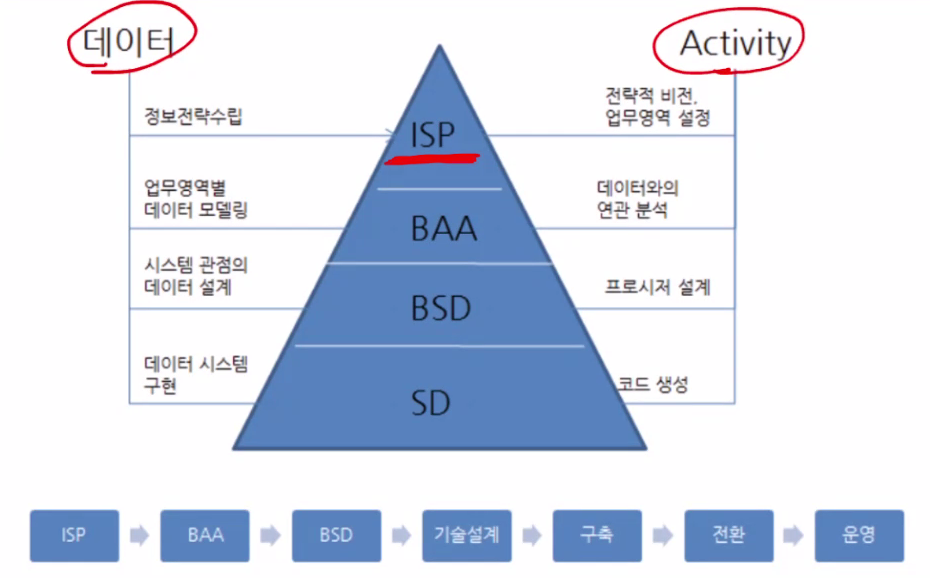
\includegraphics[scale=0.6]{22}
\newline

\subsubsection{정보 전략 계획 수립(ISP)}
- 경영 전략 분석, 업무 프로세스 분석, 현 시스템 분석/평가, Architecture 개발, 전략계획(SIS) ...

\subsubsection{업무영역 분석(BAA)}
- ISP에서 수집된 자료를 기반으로 세부적으로 확장함.
\newline
- 데이터 모델 다이어그램, 프로세스 분할 다이어그램, 프로세스/데이터 매트릭스 등 해당
\newline
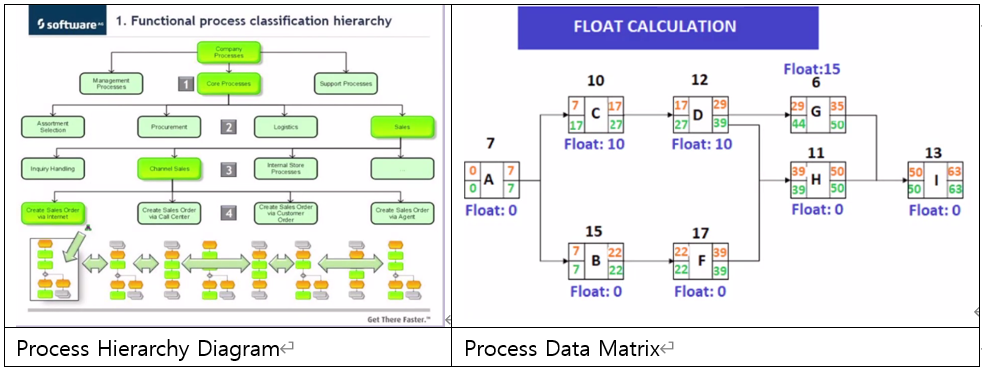
\includegraphics[scale=0.75]{23}

\subsubsection{비즈니스 시스템 설계(BSD)}
- 데이터, 시스템 구조 설계
\newline
- 기전 시스템 → 새로운 시스템으로의 전환 설계
\newline
- 엔티티 관계, 분할, 액션 다이어그램 등
\newline
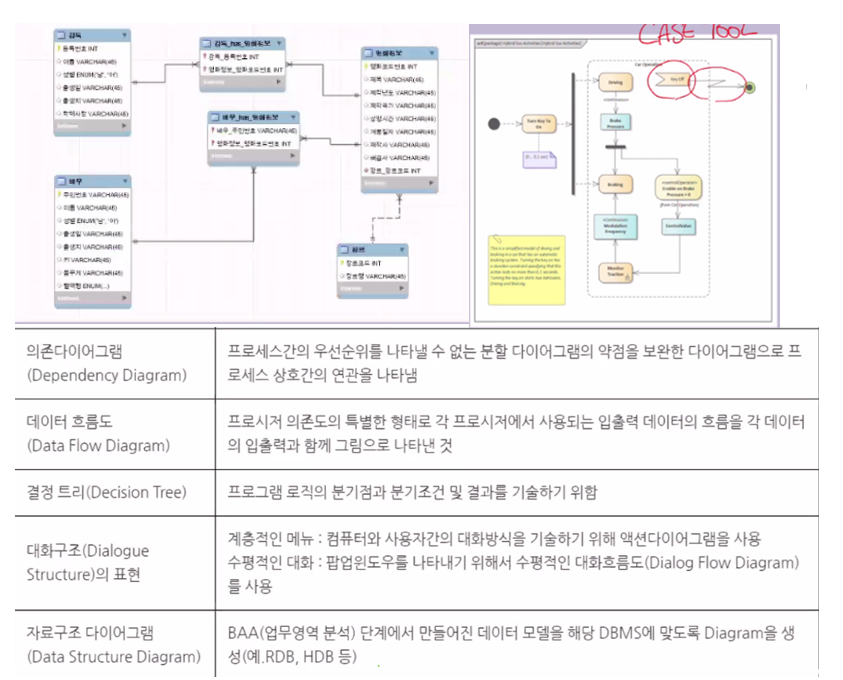
\includegraphics[scale=0.8]{24}

\subsubsection{기술 설계 및 구축}
- 물리적 DB 설계, 정보시스템 구축
\newline
- 실행 가능한 프로그램 코드 생성 및 테스트
\newline
- 이행, 설치
\newline

\subsection{한계}
i. 구조적 분석/설계 기법 ‘폭포수 모형’ 따름
\newline
ii. 복잡한 논리체계, 개발절차, 과다한 산출물
\newline
iii. 중소 규모 프로젝트에는 무리임

\newpage
% 333333333333333
\section{나선형 개발방법론}

\subsection{정의}
- 사전에 \underline{위험분석, 반복 수행, 최종 개발까지 점진적으로} 구현함.
\newline
- \textbf{단계적 소프트웨어 프로세스(Stepwise Software Process)}: 선형 순차 모델과 프로토타입의 \underline{반복적 특성}이 결합함
\newline
- 개발 중의 위험을 최소화하기 위해 \textbf{점진적으로 완벽하게} 개발함.
\newline
\newline
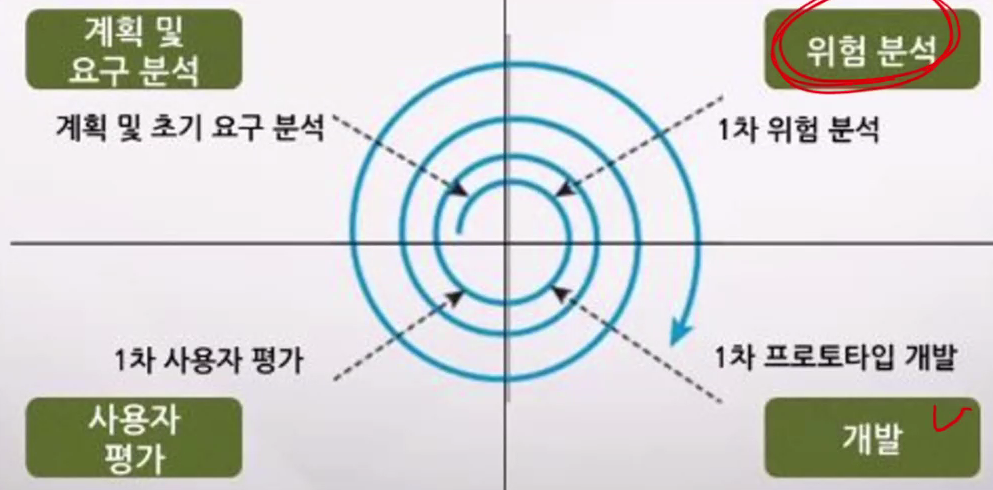
\includegraphics[scale=0.5]{31}
\newline

\subsection{특징}
- 위험을 중심으로 한 접근법이고, 개발 단계별로 위험분석을 실시함.
\newline
- \underline{위험관리 능력에 따라 성공의 여부에 영향}을 미침.
\newline
- 대규모 장기간 사업(Long Term): \underline{계획 → 위험분석 → 개발 → 평가}
\newline

\subsection{프로세스}

\subsubsection{목표 설정}
- 고객의 요구사항을 분석하고 타당성을 검토해, 프로젝트의 수행 여부를 결정함.
\newline
- 각 단계의 목표를 수립하고, 시스템 성능 등 시스템 목표를 설정하고 및 제약을 파악함.
\newline
- Cycle Processing에서 목표도 변경됨.

\subsubsection{위험 분석}
- 초기 요구사항에 근거해서 위험을 규명함.
\newline
- 프로젝트 진행 시에 고객 요구사항을 기반으로 위험 사항을 예측하고 추출해, 대처방안을 수립함.
\newline
- 의사결정(Go or No): 위험 식별 및 분석 → 위험을 최소화하고 결정함.

\subsubsection{개발}
- 위험 분석 완료 후 구축 시스템, 개발 환경에 맞는 모델을 선택함.
\newline
- 모형 선택 이후 Prototype, 완제품을 만듬.
\newline
- 여러 모델을 혼합해 개발할 수 있음.

\subsubsection{고객 평가}
- 개발, 테스트가 끝난 내용을 고객이 평가하고, 추가로 반복할 지의 여부를 결정함.
\newline
- 고객에 의해 시스템을 평가받고, 향후 목표를 계획함
\newline

\subsection{장점}
i. 고비용, 장기간의 큰 시스템 구축에 가장 현실적인 접근 방법
\newline
ii. 대규모 시스템에 적합함
\newline
iii. 모든 단계에서 위험을 고려해 사전에 위험을 방지할 수 있음
\newline
iv. 고객의 요구사항(Feedback, Commit) 등을 적용하기 쉬워 완성품의 품질과 만족도가 높음
\newline

\subsection{한계}
i. 모델이 복잡해 프로그램의 관리가 어려움
\newline
ii. \textbf{피드백 수렴, 위험분석, 의사결정 등의 시간과 비용이 높음} → 많은 고객을 대상으로 하는 상업용에 부적합함
\newline
iii. 위험 관리 전문가 필요, 접근 방법들 중에 충분한 검증이 없음


\newpage
% 444444444444
\section{프로토타이핑 개발방법론}

\subsection{정의}
- 사용자의 요구사항을 분석하기 위해, 시스템의 \underline{중요 일부분을 먼저 구현함.}
\newline
- 그 다음에 요구사항을 반영하여 \textbf{점진적(Stepwise)}으로 개발함.
\newline
- 사용자가 정보 시스템을 직접 사용해 보게 함 → 기능 수정 요구를 즉각적으로 반영함\textbf{(Reflection)} → 시스템을 재설계함\textbf{(System Reconstructure)} → 프로토타입을 재구축\textbf{(Prototype Rebuild)} → 만족 시까지 반복
\newline
- Prototype Model: 실험적, 진화적 (→ 나선형)
\newline


\subsection{특징}
- 사용자 인터페이스(UI)를 시험 제작하여, 요구사항을 도출하고 원활한 의사소통을 지원함.
\newline
- 폭포수 모델의 Feedback Weakness를 보완함.
\newline
- 고객의 요구를 상세하게 파악할 수 있음.
\newline
- Prototype을 통해 고객과 소통할 수 있음.

\subsection{프로세스}

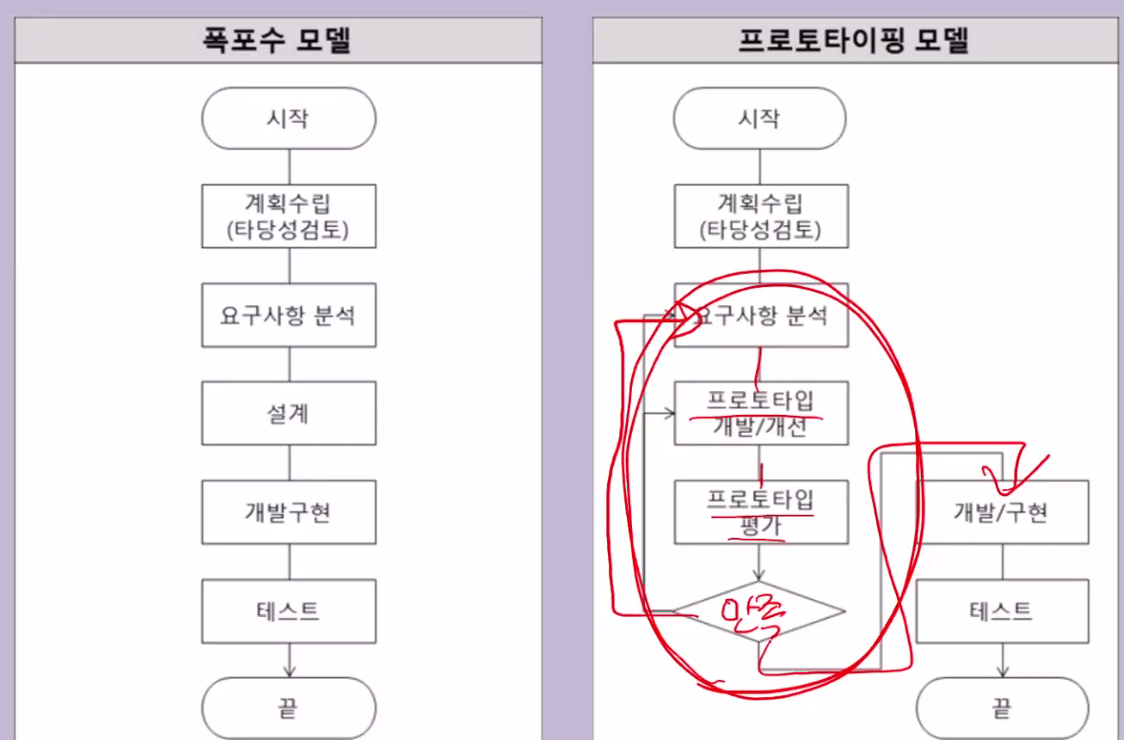
\includegraphics[scale=0.5]{41}
\newline

\subsubsection{계획 수립}
- 시스템 개발 계획을 수립하고 초기 요구사항을 수집함.
\newline
- 타당성을 검증하고 진행 여부를 결정함.

\subsubsection{요구사항 분석 및 정의}
- 고객 요구 명세서: 고객의 요구사항을 정리하고 명세화함.

\subsubsection{프로토타입 개발/개선}
- 고객에게 보여줄 (작동 가능한) 초기 Prototype 개발
\newline
- Prototype 설계서를 작성함.

\subsubsection{프로토타입 평가}
- 고객의 요구사항이 반영되었는지 개발된 Prototype을 평가하고 확인함.
\newline
- 추가 요구가 있으면 [4.3.2]로 돌아가고, 없으면 진행함.
\newline
- Prototype 평가서를 작성함.

\subsubsection{개발/구현}
- Prototype을 실제 System으로 구현함.
\newline
- 실행 파일, 테스트 계획 및 결과서를 작성함.

\subsubsection{테스트}
- 전체적 시스템을 구현하고 완전한 시스템으로써의 테스트를 실행함.
\newline

\subsection{장점}
i. 고객의 요구사항(Feedback, Commit) 등을 적용하기 쉬워 완성품의 품질과 만족도가 높음.
\newline
ii. Prototype: 개발자/고객간 의사소통이 원활해 요구사항의 수용이 빠름.
\newline
iii. 오류를 초기에 발견하고 변경하기에 용이함.
\newline

\subsection{한계}
i. 유지보수에 필수적인 시스템의 문서화 과정이 지나치게 축소되거나 생략될 수 있음.
\newline
ii. 변경이 계속될수록 시간과 비용이 많이 듬.
\newline
iii. Prototype이 폐기될 시 비경제적이고, 완제품과 오인될 수 있음.



\newpage
% 55555555555555
\section{반복적 개발방법론}

\subsection{정의}
- 요구사항이나 제품의 일부분만을 개발/반복해 최종 요구 사항에 부합하는 시스템을 완성함.
\newline
- \textbf{Prototype Model도 Repetitive Model에 해당함.}
\newline
- Repetitive Model: \textbf{증분형/점진적(Incremental), 진화형(Evolutional).}
\newline

\subsection{증분형 모델(Incremental)}

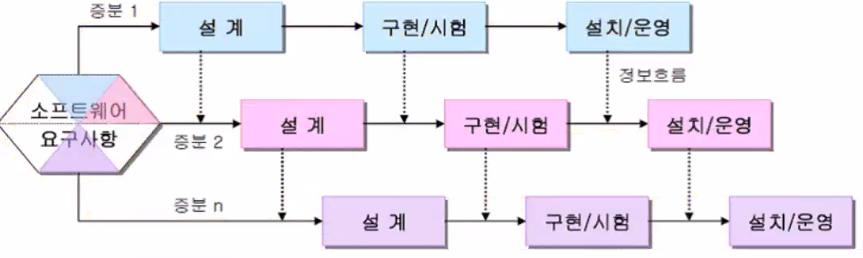
\includegraphics[scale=0.6]{51}
\newline
- 한 시스템을 기능별로 여러 서브시스템으로 분리함.
\newline
- \underline{분리한 서브 시스템을 하나씩 완성 후 결합함.} (증분형 모델)
\newline
- 전체 시스템의 일부 가능을 Sub-System화, 반복적으로 개발/추가해서 최종 완성품을 제작하는 방법론임.
\newline
- Sub-System 병행 개발로 개발 기간을 단축할 수 있음.
\newline
- 증분이 너무 많아지면 관리가 힘듬.
\newline
- \underline{폭포수 모델의 변형형임.}


\subsection{진화형 모델(Evolutional)}
- \textbf{하나의 시스템(Prototype)}을 만든 후, \underline{지속적으로 추가 기능을 붙여} 릴리즈마다 기능을 추가/개선함 → 최종적으로 완벽한 시스템으로 개발
\newline
- 작은 눈덩이를 굴려 큰 눈덩이를 만드는 형태임.
\newline
- Prototype의 특징과 유사하며 단점을 보완함.
\newline
- 요구사항을 명확히 정의하기 힘들 때 사용함.
\newline
- 증분 설계가 다음 설계에 반영됨.
\newline
- \textbf{Re-using Prototype → System Evolution}
\newline
- 진화 단계에 따라 릴리즈 버전을 명확히 표기해야 함.
\newline
\newline
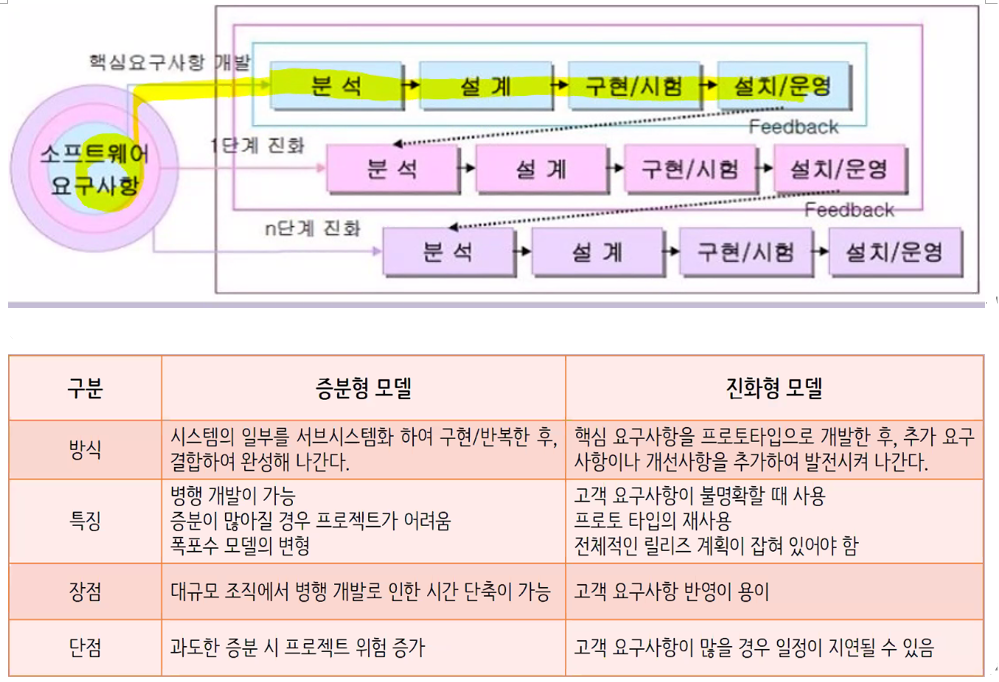
\includegraphics[scale=0.75]{52}


\newpage
% 666666666666666
\section{객체지향 개발방법론}

\subsection{정의}
- 현실의 개체를 \textbf{속성(Data)}와 \textbf{Method(Operator)}로 구성된 \textbf{'객체(Object)'}로 표현함.
\newline
- Independant Object들이 Message 교환을 통해 상호작용(Interaction)함.
\newline
\newline
- 객체지향의 구성 요소:

- i) \textbf{객체(Object)}: 속성(Attribute)와 메소드(Method)가 결합된 클래스의 인스턴스.

- ii) \textbf{클래스(Class)}: 하나 이상의 유사한 객체를 묶어 공통된 특성을 표현한 데이터 추상화(Data Abstract).

- iii) \textbf{메소드(Method)}: 객체가 메시지를 받아 실행해야 할 객체의 구체적인 연산.

- iv) \textbf{메시지(Message)}: 객체들 간에 상호작용하는데 사용되는 수단.
\newline
\newline
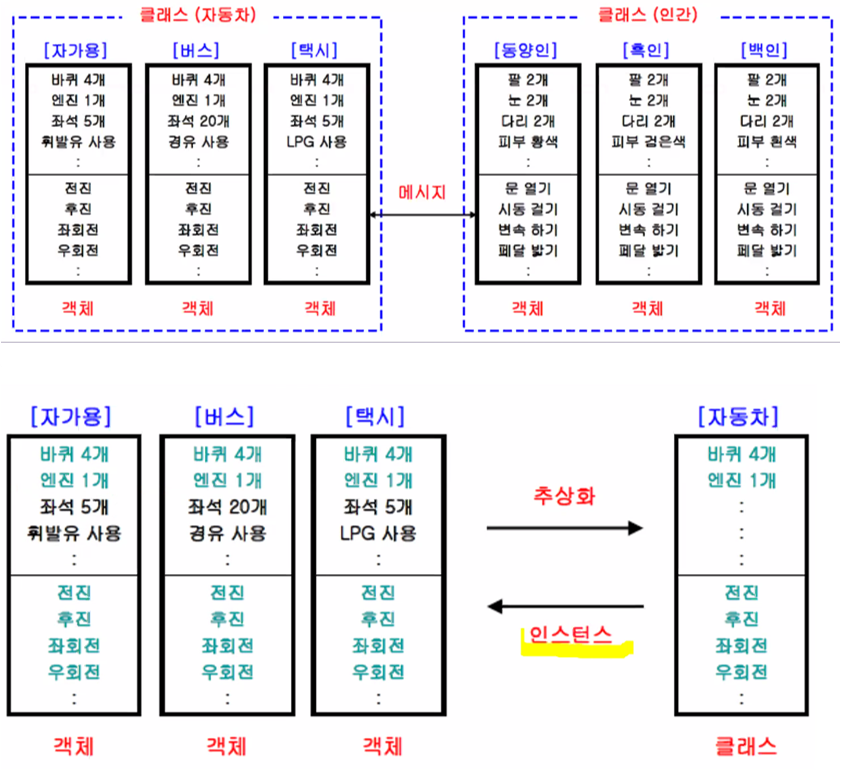
\includegraphics[scale=0.8]{53}
\newline

\subsection{특징}
\subsubsection{캡슐화 (Encapsulation)}
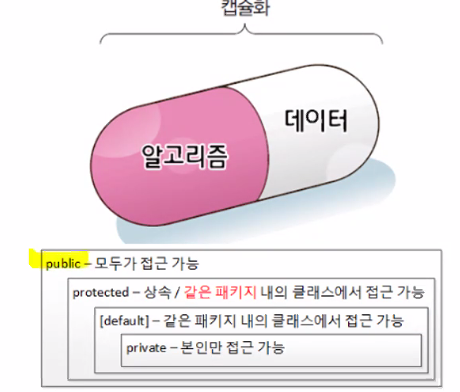
\includegraphics[scale=0.7]{54}
\newline
- 객체 내부 문제는 숨기고, \underline{외부와 상호작용(인터페이스)에 관계된 것만 개방함.}
\newline
- 관련 Data, Algorithm들이 하나의 형태로 정의됨.

\subsubsection{추상화 (Abstract)}
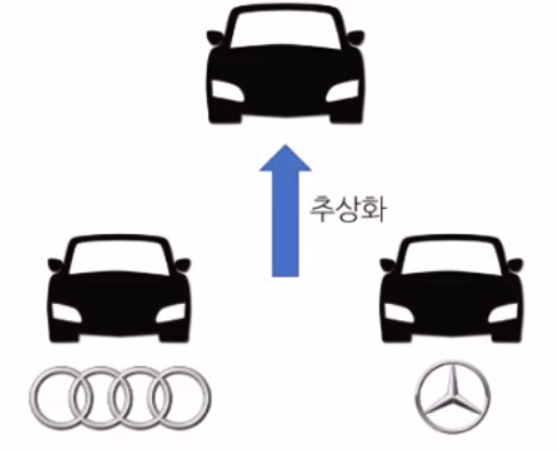
\includegraphics[scale=0.8]{55}
\newline
- 어떤 영역에서 필요한 속성/행동을 추출함.
\newline
- \underline{사물의 공통적인 특징}을 파악해 하나의 개념(집합)으로 다룸.
\newline
- 클래스를 이용해 추상화를 실현함.
\newline
- 객체 중심의 \underline{안정되고 자연스러운 현실 세계의 모델}을 구축할 수 있음.

\subsubsection{다형성 (Polymorphism)}
- 동일한 외부 명령에 대해 \underline{각 개체가 다른 방식으로 명령을 수행함.}
\newline
- \textbf{오버로딩(Over-Loading)}: 클래스 내 동일 메소드가 (다른 Parameter로) 중복 정의된 것.
\newline
- \textbf{오버라이딩(Over-Riding)}: 부모 클래스에서 정의된 메소드를 자식 이 재정의하는 것.

\subsubsection{정보 은닉 (Information Hiding)}
- 캡슐화된 항목이 \underline{다른 객체에게 보이지 않게 함.}
\newline
- 블랙박스 역할: Data/Method를 숨기고, 객체의 사용자와 제공자 간의 역할을 분리함.
\newline
- Interface로 접근: 객체 내부의 자료 구조를 몰라도 객체를 쉽게 이용 가능함.
\newline
- 자료구조 변이의 용이: 제공자가 내부의 자료 구조를 변경해도 사용에 영향이 없음.
\newline
- Module Independency 높임.

\subsubsection{상속성 (Inheritance)}
- 하위 클래스에게 \underline{자신의 속성과 메소드를 사용할 수 있도록 허용함.}
\newline
- \textbf{단일 상속}: super/sub 클래스의 관계를 유지함.
\newline
- \textbf{다중 상속}: 하나의 클래스가 하나 이상의 클래스로부터 상속받음.
\newline
- 개별 클래스를 상속 관계로 묶음 → 클래스 사이 전체 구조 이해에 용이함.
\newline
- 재사용성 증대 (Over-Loading 피하고 Reuse) → \textbf{Duplicated Redefinition을 방지함.}
\newline

\subsection{프로세스}

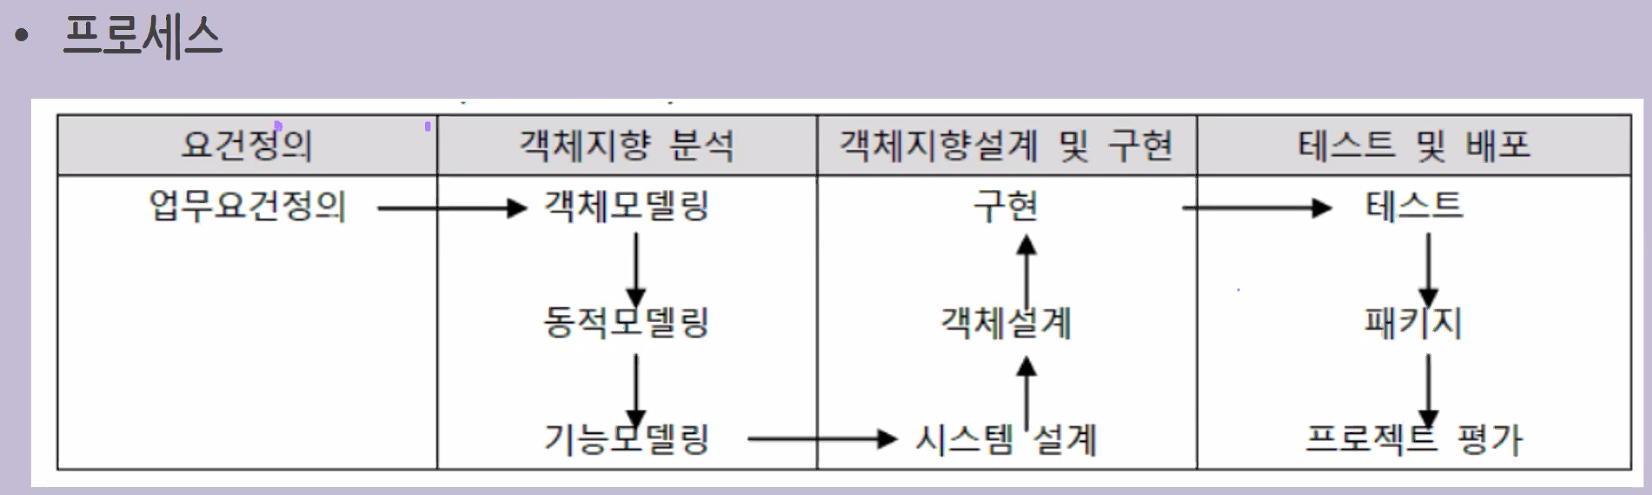
\includegraphics[scale=0.4]{56}
\newline

\subsubsection{객체 모델링(Object Modeling)}
- 요구사항 분석 → 객체 추출 → 객체 특성과 객체 사이 관계 규명
\newline
- 산출물: \textbf{객체 다이어그램(Object Diagram)}

\subsubsection{동적 모델링(Dynamic Modeling)}
- 시간의 흐름에 따라 객체 사이의 변화를 조사함.
\newline
- 산출물: \textbf{상태도 (Phase Diagram)}

\subsubsection{기능 모델링(Functional Modeling)}
- 입력에 대한 처리 결과들에 대해 확인함.
\newline
- 산출물: \textbf{자료 흐름도 (DFD, Data Flow Diagram)}

\subsubsection{객체 설계(Object Constructing)}
- 객체 모형을 구체화시키고, 자료구조와 알고리즘을 구현함.

\newpage
% 7777777777777
\section{컴포넌트(CBD) 개발방법론}

\subsection{개요}
\subsubsection{등장 배경}
- 기업 환경 변화에 따라 \underline{SW가 대형화, 복잡화됨.}
\newline
- 복잡성과 유지보수 비용이 증가하였고, 개발 생산성 향상 및 높은 질의 SW에 대한 요구가 등장함.
\newline
- 객체지향(Object-Oriented) 개발방법론은 단일 언어로 개발하고 \underline{수시로 모듈을 수정해 재컴파일}해야하는 불편함이 있음.

\subsubsection{컴포넌트(CBD) 정의}
- \textbf{모듈(Module)}: 함수가 합쳐 기능을 수행함.
\newline
- \textbf{컴포넌트(CBD)}: 모듈을 합쳐 기능을 수행함.
\newline
- SW 시스템에서 독립적인 업무나 기능을 모듈로써 수행함.
\newline
- 일체형 구축이 아니며, \textbf{레고 블록처럼 요소 별로 부품화하여 구축함.}
\newline
- 각 기능을 분리해 개발한 여러 컴포넌트를 제작 후 재조립함 → 시스템과 SW에서 재사용하기 용이함.
\newline


\subsection{특징}
- 독립적인 SW Module임 → \textbf{No Dependency.}
\newline
- \textbf{구현(Implementation), 명세화(Specification), 패키지화, 배포 가능}해야 함.

C1\footnote{조건(Condition)}. 소스 코드가 아닌 \underline{실행 코드 기반으로 구현 완료}해야 함.

C2. 해당 CBD의 \underline{용도, 유형, 기술표준, Interface 등의 정보}를 명세화해야 함.

C3. 사용자가 필요한 기능만 Package한 CBD를 \underline{재사용할 수 있도록 독립 배포}해야 함.
\newline
- 하나의 CBD는 하나 이상의 클래스로 구성될 수 있음.
\newline
- Interface로만 접근 가능함 → \textbf{캡슐화(Encapsulated)}
\newline

\subsection{프로세스}

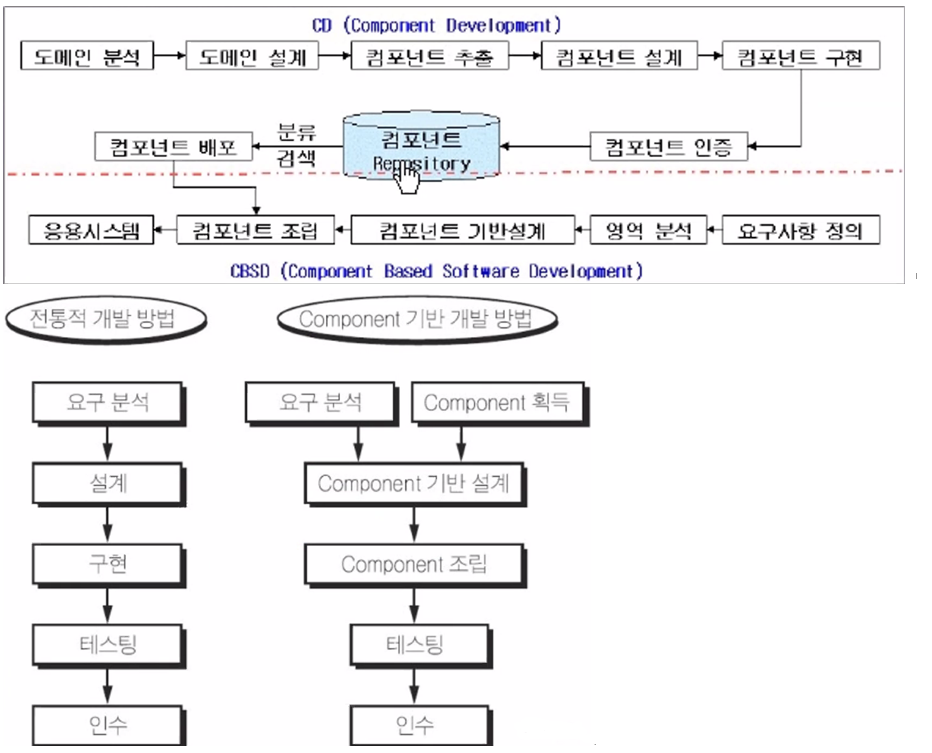
\includegraphics[scale=0.65]{57}
\newline

\subsection{장점}
i. 미리 구현된 CBD 조립 → 유연한 SW 구축이 가능함.
\newline
ii. \underline{well-defined, verified된 CBD 사용} → 개발기간이 단축되고 품질 수준이 향상됨.
\newline
iii. 자원의 재사용성이 확대됨 → 개발비용이 감소하고 생산성이 증대됨.
\newline
iv. 테스트된 CBD 사용 → 리스크가 감소함.
\newline
v. 변경이 용이하고 안정적으로 대처할 수 있음.
\newline

\subsection{한계}
i. CBD들이 이질적인 기술 환경에서 개발됨.
\newline
ii. 통합을 염두하고 시스템 개발을 관리해야 함.
\newline
iii. 기존 CBD가 시스템의 비즈니스 요구 사항을 적절히 충족하지 못할 수도 있음.
\newline
iv. CBD의 평가 및 인증 환경이 미흡함.
\newline
\newline
\newline


\section{마치면서}
\textbf{김지훈}입니다.
\newline
koTeX로 써보는 건 처음입니다.
\newline
감사합니다. 

\end{document}